\documentclass[10pt]{beamer}



\usetheme[progressbar=frametitle]{metropolis}
\usepackage{appendixnumberbeamer}

\usepackage{booktabs}
\usepackage[scale=2]{ccicons}

\usepackage{pgfplots}
\usepgfplotslibrary{dateplot}

\usepackage{xspace}


\usepackage[brazil]{babel}
\usepackage[utf8]{inputenc}
\usepackage{amsmath}
\usepackage{amsfonts}
\usepackage{amssymb}
\usepackage{mathtools}
\usepackage{physics}
\usepackage{calligra}

\DeclareMathAlphabet{\mathcalligra}{T1}{calligra}{m}{n}
\DeclareFontShape{T1}{calligra}{m}{n}{<->s*[2.2]callig15}{}
\newcommand{\scripty}[1]{\mathcalligra{#1}\,}
\newcommand{\boldscripty}[1]{\pmb{\mathcalligra{#1}}\,}
\newcommand{\hscripty}[1]{\vu*{\boldscripty{#1}}}


\newcommand*{\dt}[1]{%
  \accentset{\mbox{\large\bfseries .}}{#1}}
\newcommand*{\ddt}[1]{%
  \accentset{\mbox{\large\bfseries .\hspace{-0.25ex}.}}{#1}}
\newcommand*{\dddt}[1]{%
  \accentset{\mbox{\large\bfseries .\hspace{-0.25ex}.\hspace{-.20ex}}}{#1}}
\newcommand*{\dnt}[2][4]{\dt{#2}^{\tiny(#1)}}


\title{Mapeamento Clássico-Quântico - Estudando o Emaranhamento Quântico  simulando Modelos Clássicos para o Modelo de Ising }
\author{Alex Enrique Crispim}
\date{\today}
%\date{}


\begin{document}
\maketitle

\begin{frame}{Tópicos}
	\begin{itemize}
		\item Conceitos preliminares de Termodinâmica e Mecânica Estatística 
		\item O Modelo de Ising Clássico e o Modelo Quântico de Ising
		\item A ideia do mapeamento clássico-quântico
		\item Monte Carlo e Algoritmo de Metropolis
		\item Cadeias de Markov e Teoria Ergódicas
		\item Amostrando-se o espaço de fase e calculando-se médias
		\item Calculando-se observáveis clássicos
		\item Calculando-se observáveis quânticos via observáveis clássicos
		\item Transições quânticas de fase e o emaranhamento quântico	
	\end{itemize}
\end{frame}


%\begin{frame}{Termodinâmica e Mecânica Estatística - Dinâmica}

%\end{frame}



\begin{frame}{Termodinâmica e Mecânica Estatística - Dinâmica}
	- Dinâmica de sistemas $\to$ minimização da energia e maximização da entropia
\end{frame}

\begin{frame}{Termodinâmica e Mecânica Estatística - Dinâmica}
	- Dinâmica de sistemas $\to$ minimização da energia e maximização da entropia $\Leftrightarrow$ \textit{Minimização da Energia livre $F$}\\
	
	\begin{equation*}
		F = U - TS
	\end{equation*}
		\begin{equation*}
		dF = dU - TdS
	\end{equation*}

\end{frame}

\begin{frame}{Termodinâmica e Mecânica Estatística - Dinâmica}
	\begin{equation*}
		F = U - TS
	\end{equation*}
	
	$F$ é uma função de estado. 	
	
\end{frame}

\begin{frame}{Termodinâmica e Mecânica Estatística - Dinâmica}
	$F$ é uma função de estado.  \\
	\begin{equation*}
		F = U - TS
	\end{equation*}
	

	
\end{frame}

\begin{frame}{Termodinâmica e Mecânica Estatística - Dinâmica}
	$F$ é uma função de estado.  \\
	\begin{equation*}
		F = U - TS
	\end{equation*}
	
	Energia livre $\to$ Peso de Boltzmann
	\begin{equation*}
		P(E) = e^{-\beta E} \qc \beta = \frac{1}{kT}.
	\end{equation*}
	
\end{frame}


\begin{frame}{Termodinâmica e Mecânica Estatística - Dinâmica}
	Distribuição de Boltzmann\\
	\begin{equation*}
		\mu_\beta (H(x)) = \frac{1}{Z} e^{-\beta H(x)} \qc Z = \int e^{-\beta H(x)} dx
	\end{equation*}
	
\end{frame}

\begin{frame}{Termodinâmica e Mecânica Estatística - Dinâmica}
	Calculo de observáveis macroscópicos por meio da medida $\mu_\beta$
	\begin{equation*}
		\ev{M(x)}_T = \int  M(x) e^{-\beta H(x)} dx.
	\end{equation*}

	
\end{frame}



\begin{frame}{O Modelo de Ising Clássico e o Modelo Quântico de Ising}
	- 1940 \\
	- Wilhelm Lenz $\to$ Ernest Ising
	\begin{figure}
		\center
		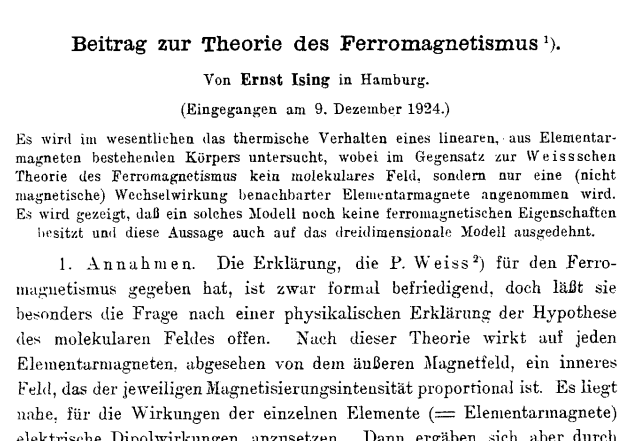
\includegraphics[scale=.4]{IsingPaper.png}
	\end{figure}
\end{frame}

\begin{frame}{O Modelo de Ising Clássico e o Modelo Quântico de Ising}
	- Estudar o ferromagnetismo \\
	\begin{figure}[h]
		\center
		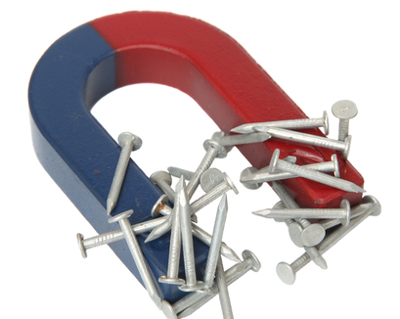
\includegraphics[scale=.25]{ferromag.jpg}
	\end{figure}
	\scriptsize fonte da figura: alunosonline.uol.com.br
	\normalsize
	
	- Spins \\
	- Transição de fase ordem$-$desordem.
	\begin{figure}
		\center
		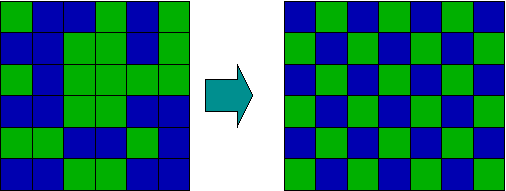
\includegraphics[scale=.3]{Ordering.png}
	\end{figure}

\end{frame}

\begin{frame}{O Modelo de Ising Clássico e o Modelo Quântico de Ising}
	Hamiltoniana (clássica) de Ising
	\begin{equation*}
		H = - \sum_{\ev{i,j}} J_{ij} \sigma_i \sigma_j - \sum_i B_i \sigma_i 
	\end{equation*}
	\\
	Rede quadrada
	\begin{figure}[h]
		\center
		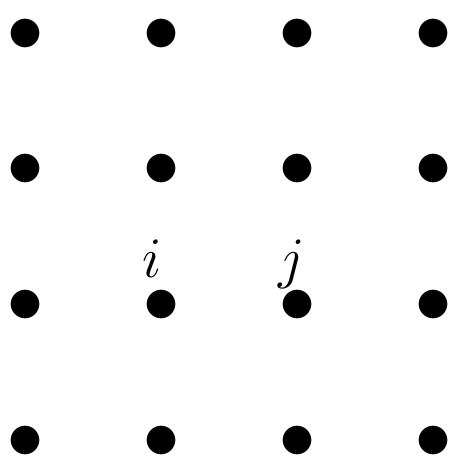
\includegraphics[scale=.2]{rede2d.png}	
	\end{figure}

\end{frame}

\begin{frame}{O Modelo de Ising Clássico e o Modelo Quântico de Ising}
	- Model 1D 
	\begin{figure}[h]
		\center
		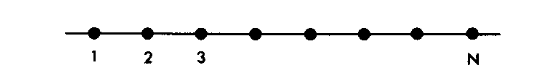
\includegraphics[scale=.3]{1dIsing.png}
	\end{figure}
	
	\begin{equation*}
		M_0 = \lim_{H \to 0^+} M(H, T) \qc M(H,T) = \ev{ \sigma_j }
	\end{equation*}
	
\end{frame}

\begin{frame}{O Modelo de Ising Clássico e o Modelo Quântico de Ising}
	- Model 1D 
	\begin{figure}[h]
		\center
		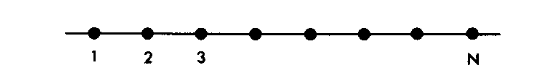
\includegraphics[scale=.3]{1dIsing.png}
	\end{figure}
	
	\begin{equation}
		M(H, T) = \frac{e^{\beta J} \sinh(\beta H)}{e^{2\beta J}\sinh[2](\beta H) + e^{2-\beta J}}.	
	\end{equation}		
	\begin{equation*}
		\lim_{H \to 0^+} M(H, T) = 0 \qc \forall T > 0.
	\end{equation*}
	
\end{frame}


\begin{frame}{O Modelo de Ising Clássico e o Modelo Quântico de Ising}
	Segundo Ising, \\
	
	\begin{center}
		Model 1D sem transição $\Rightarrow$ Modelo de qualquer dimensão sem transição 
	\end{center}
	\begin{figure}[h]
		\center
		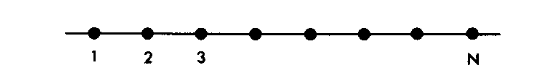
\includegraphics[scale=.3]{1dIsing.png}
	\end{figure}
	
	\begin{equation*}
		\lim_{H \to 0^+} M(H, T) = 0 \qc \forall T > 0.
	\end{equation*}
	
\end{frame}


\begin{frame}{O Modelo de Ising Clássico e o Modelo Quântico de Ising}

	Peirls, 1936 - Transição de fase para 2D.
	\begin{figure}[h]
		\center
		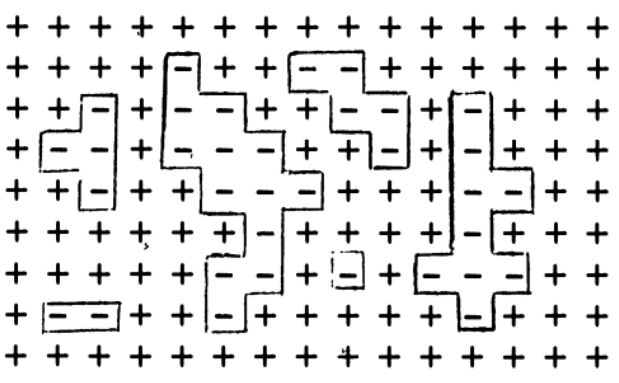
\includegraphics[scale=.3]{2d.png}
	\end{figure}
\end{frame}

\begin{frame}{O Modelo de Ising Clássico e o Modelo Quântico de Ising}
	Onsager 1944 - Solução exata
	
	\begin{equation*}
		\beta_c J = \frac{\ln(1+\sqrt{2})}{2}
	\end{equation*}
	
	- Primeiro modelo a apresentar transições de fase\\
	- Início de um novo marco no estudo de sistemas fortemente correlacionados
\end{frame}


\begin{frame}{A ideia do mapeamento clássico-quântico}
	Hamiltoniana clássica bidimensional ($B = 0$).
	\begin{equation*}
		H = - J_1 \sum_{i, j} \sigma_i^j \sigma_{i+1}^j  - J_2 \sum_{i,j} \sigma_i^j \sigma_i^{j+1} 
	\end{equation*}
	\\
	Hamiltoniana quântica unidimensional
	\begin{equation*}
		\hat{H} = -J \sum_i \hat{\sigma}^z_i \hat{\sigma}^z_{i+1} + \lambda \hat{\sigma}^x_i		
	\end{equation*}
	\\
	$$Z_q \mapsto Z_{cl}. $$
\end{frame}

\begin{frame}{A ideia do mapeamento clássico-quântico}
	$$Z_q \mapsto Z_{cl}. $$
	\\
	\begin{center}
		Observáveis quânticos $\mapsto$ observáveis clássicos.
	\end{center}
\end{frame}

\begin{frame}{A ideia do mapeamento clássico-quântico}
	$$\text{direção } y \to \text{tempo} (complexo) $$
	\begin{figure}[h]
		\center
		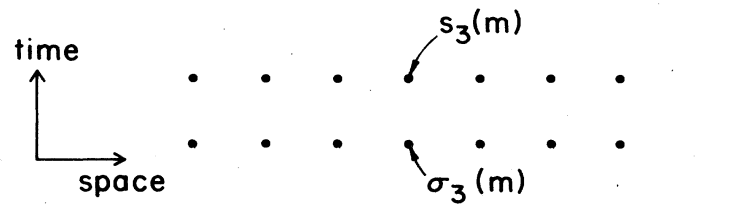
\includegraphics[scale=.3]{2dmapping.png}
	\end{figure}
	\begin{center}
		Espaço Euclidiano (2+0) $\mapsto$ Espaço de Minkowski (1+1)
	\end{center}
	
\end{frame}


	
\begin{frame}{A ideia do mapeamento clássico-quântico}
	$$Z_q \mapsto Z_{cl}. $$
	\\
	\begin{center}
		- Observáveis quânticos $\mapsto$ observáveis clássicos.\\
		- Cálcular os observáveis clássicos e determinar o análogo quântico. 
	\end{center}
\end{frame}


\begin{frame}{Monte Carlo e o Algoritmo de Metrópolis}
	- Cálculo de probabilidades usando estatística
	- Cálculo de quantidades estatísticas usando probabilidade	
\end{frame}

\begin{frame}{Monte Carlo e o Algoritmo de Metrópolis}
	- Cálculo de probabilidades usando estatística
	- Cálculo de quantidades estatísticas usando probabilidade	
	\begin{figure}[h]
		\center
		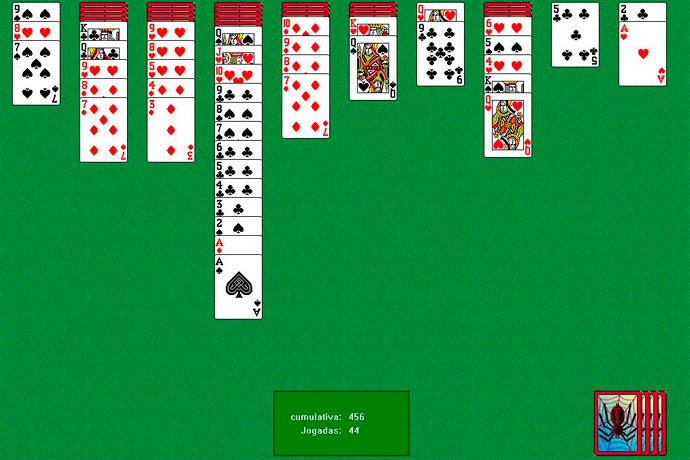
\includegraphics[scale=.25]{paci.jpg}
	\end{figure}
\end{frame}

\begin{frame}
	\begin{figure}[h]
		\center
		
\includegraphics[scale=.3]{hearthstoneLogo.png}
	\end{figure}
	\begin{figure}[h]
		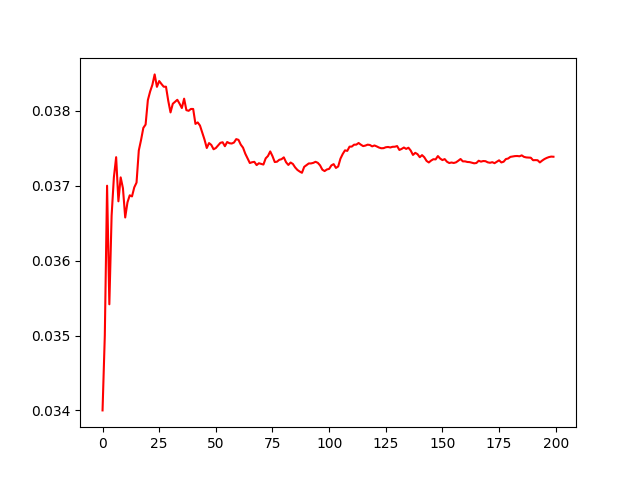
\includegraphics[scale=.4]{SimHS.png}
	\end{figure}
\end{frame}





\begin{frame}{Monte Carlo e o Algoritmo de Metrópolis}
	Cálculo do $\pi$
	\begin{figure}[h]
		\center
		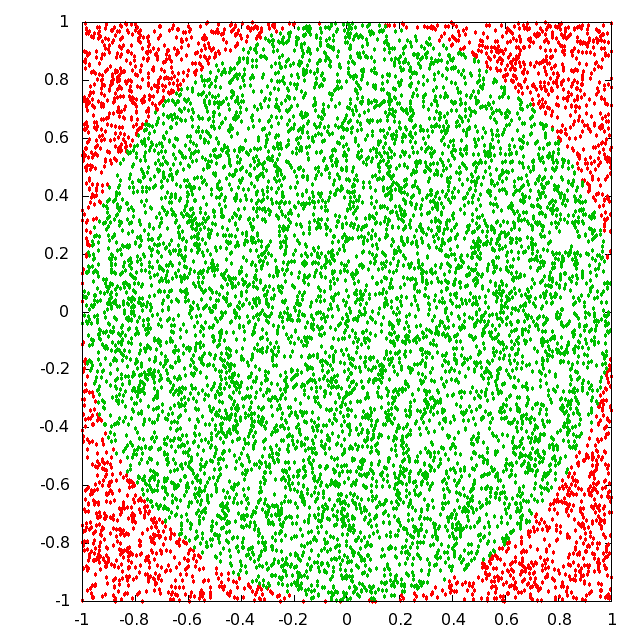
\includegraphics[scale=.25]{pi.png}
	\end{figure}
\end{frame}

\begin{frame}{Monte Carlo e o Algoritmo de Metrópolis}
	- Uso do Monte Carlo para o cálculo dos observáveis clássicos \\
	- Como?
	
\end{frame}

\begin{frame}{Monte Carlo e o Algoritmo de Metrópolis}
	- Uso do Monte Carlo para o cálculo dos observáveis clássicos \\
	- Como?

	\vspace*{1cm}
	- Algoritmo de Metropolis	
\end{frame}

\begin{frame}{Cadeias de Markov e Teoria Ergódicas}
	\textbf{Cadeias de Markov}\\
	
	$\Gamma = \Gamma_1, \Gamma_2, ...$
	\begin{equation*}
		\Gamma_k = \{ \sigma_k \}
	\end{equation*}
	
	- Probabilidade de transição
	\begin{equation*}
		\Gamma_i \xrightarrow[]{ p_{ij} } \Gamma_j \qc \forall (i, j)
	\end{equation*}
\end{frame}


\begin{frame}{Cadeias de Markov e Teoria Ergódicas}
	\textbf{Cadeias de Ergódicas}\\
	\begin{equation*}
		p_{ij}^{(n)} = \mu(\Gamma_{m+n} = 	\{ \sigma_j \} \vert \Gamma_m = \{ \sigma_i \}) > 0.	
	\end{equation*}		
	
	\textbf{Teorema}
	\begin{equation*}
		\pi_j = \lim_{n \to \infty} p_{ij}^{(n)} \text{ existe e independe de } i.
	\end{equation*}

\end{frame}


\begin{frame}{Cadeias de Markov e Teoria Ergódicas}
	\textbf{Cadeias de Ergódicas}\\
	\begin{equation*}
		p_{ij}^{(n)} = \mu(\Gamma_{m+n} = 	\{ \sigma_j \} \vert \Gamma_m = \{ \sigma_i \}) > 0.	
	\end{equation*}		
	
	\textbf{Teorema}
	\begin{equation*}
		\pi_j = \lim_{n \to \infty} p_{ij}^{(n)} \text{ existe e independe de } i.
	\end{equation*}

	- $\pi_j$ independe do estado inicial!
\end{frame}


\begin{frame}{Cadeias de Markov e Teoria Ergódicas}
	\textbf{Cadeias de Ergódicas}\\
	\begin{equation*}
		p_{ij}^{(n)} = \mu(\Gamma_{m+n} = 	\{ \sigma_j \} \vert \Gamma_m = \{ \sigma_i \}) > 0.	
	\end{equation*}		
	
	\textbf{Teorema}
	\begin{equation*}
		\pi_j = \lim_{n \to \infty} p_{ij}^{(n)} \text{ existe e independe de } i.
	\end{equation*}

	- $\pi_j$ independe do estado inicial! \\
	- Modelo de Ising
\end{frame}

\begin{frame}{Cadeias de Markov e Teoria Ergódicas}
	\textbf{Teorema Ergódico}
	\begin{theorem}
		Seja $(\mathcal{X}, \Sigma, \mu, T)$ um sistema dinâmico que preserva medida e $f$ uma função $\mu$-integrável. Então, as seguintes médias
		\begin{equation*}
			\text{Média temporal: } \hat{f}(x) = \lim_{n \to \infty} \frac{1}{n} \sum_{k=0}^{n-1} f(T^k x),
		\end{equation*}
		\begin{equation*}
			\text{Média espacial: } \bar{f}(x) = \frac{1}{\mu(\mathcal{X})} \int f \dd{\mu},
		\end{equation*}
Se igualam.

	\end{theorem}
	
\end{frame}


\begin{frame}{Cadeias de Markov e Teoria Ergódicas}
	\textbf{Teorema Ergódico}
	\begin{theorem}
		Seja $(\mathcal{X}, \Sigma, \mu, T)$ um sistema dinâmico que preserva medida e $f$ uma função $\mu$-integrável. Então, as seguintes médias
		\begin{equation*}
			\text{Média temporal: } \hat{f}(x) = \lim_{n \to \infty} \frac{1}{n} \sum_{k=0}^{n-1} f(T^k x),
		\end{equation*}
		\begin{equation*}
			\text{Média espacial: } \bar{f}(x) = \frac{1}{\mu(\mathcal{X})} \int f \dd{\mu},
		\end{equation*}
Se igualam.

	\end{theorem}
	
	\begin{equation*}
		\boxed{ \text{\large Amostrar no espaço de fase se iguala a amostrar no tempo!} }
	\end{equation*}
\end{frame}

\begin{frame}{Amostrando-se o espaço de fase e calculando-se médias}
	Pelo Teorema Ergódico. 
	
	\begin{equation*}
		\ev{ M } = \frac{1}{M} \sum_{i = 1}^M M(\{ \sigma_i \}).
	\end{equation*}


\end{frame}

\begin{frame}{Amostrando-se o espaço de fase e calculando-se médias}
	Pelo Teorema Ergódico. 
	
	\begin{equation*}
		\ev{ M } = \frac{1}{M} \sum_{i = 1}^M M(\{ \sigma_i \}).
	\end{equation*}

	Questão: $M(\{ \sigma_i \})$...

\end{frame}


\begin{frame}{Amostrando-se o espaço de fase e calculando-se médias}
	Pelo Teorema Ergódico. 
	
	\begin{equation*}
		\ev{ M } = \frac{1}{M} \sum_{i = 1}^M M(\{ \sigma_i \}).
	\end{equation*}

	Questão: $M(\{ \sigma_i \})$... \\
	\ \ \ $ \hookrightarrow $ Dinâmica da rede.
\end{frame}


\begin{frame}{Amostrando-se o espaço de fase e calculando-se médias}
	Equação de balanceamento
	\begin{equation*}
		\mu_\beta (\{ \sigma_i \} ) \mathcal{A} (\{ \sigma_i \} \to \{ \sigma_j \}) = \mu_\beta(\{ \sigma_j \}) \mathcal{A}(\{ \sigma_j \} \to \{ \sigma_i \}). 
	\end{equation*}


\end{frame}


\begin{frame}{Amostrando-se o espaço de fase e calculando-se médias}
	Equação de balanceamento
	\begin{equation*}
		\mu_\beta (\{ \sigma_i \} ) \mathcal{A} (\{ \sigma_i \} \to \{ \sigma_j \}) = \mu_\beta(\{ \sigma_j \}) \mathcal{A}(\{ \sigma_j \} \to \{ \sigma_i \}). 
	\end{equation*}

	\begin{equation*}
		\mathcal{A} = 
		\begin{cases}
			1,   & \delta H \leq 0, \\
			e^{-\delta H},   &\delta H > 0.
		\end{cases}
	\end{equation*}

	$\mathcal{A} \to $ Metropolis + Monte Carlo
\end{frame}


\begin{frame}{Calculando-se observáveis clássicos}
	Método de Monte Carlo \\
	
	\ \ \ - Algoritmo de Metropolis

\end{frame}

\begin{frame}{Calculando-se observáveis clássicos}
	\textbf{Algoritmo de Metropolis} \\
	
	\ \ \- Inicializa a rede. 
	\begin{figure}[h]
		\center
		
\includegraphics[scale=.2]{initLattice.png}	
	\end{figure}

\end{frame}

\begin{frame}{Calculando-se observáveis clássicos}
	\textbf{Algoritmo de Metropolis} \\
	
	\ \ \- Inicializa a rede. \\
	\ \ \ - Escolhe uma posição aleatória
	\begin{figure}[h]
		\center
		
\includegraphics[scale=.2]{initLattice.png}	
	\end{figure}

\end{frame}

\begin{frame}{Calculando-se observáveis clássicos}
	\textbf{Algoritmo de Metropolis} \\
	
	\ \ \- Inicializa a rede. \\
	\ \ \ - Escolhe uma posição aleatória \\
	\ \ \ - $\text{Se } \Delta H \leq 0 \text{ ou } R < e^{-\beta \Delta H}, \text{ flipa o spin} $ (R = \texttt{random()} $\in [0, 1)$).
	\begin{figure}[h]
		\center
		
\includegraphics[scale=.2]{initLattice.png}	
	\end{figure}

\end{frame}





\begin{frame}
	Modelo de Ising se liga a diversas outras áreas. \\
	- Teoria de Campos. \\
	 \ \ - Conformal Field Theory. \\
	- Fermions de Majorana. \\
	...
\end{frame}



\end{document}